\documentclass{article}
\usepackage{tikz}
\usetikzlibrary{arrows, shapes, positioning}
\usepackage{bm}
%\tikzstyle{nodeobserved} = [circle, minimum size = 10mm, thick, draw =black!80]
\usetikzlibrary{external}
\usepackage{amsmath}
\usepackage{pgfplots}
\usepackage{graphicx}

\tikzexternalize

\begin{document}

\begin{figure}
    \centering
    \tikzsetnextfilename{empty}
    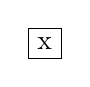
\begin{tikzpicture}
        \node[draw] (x) at (0,0) {x};
    \end{tikzpicture}
\end{figure}

\begin{figure}
    \centering
    \tikzsetnextfilename{overfitting}
    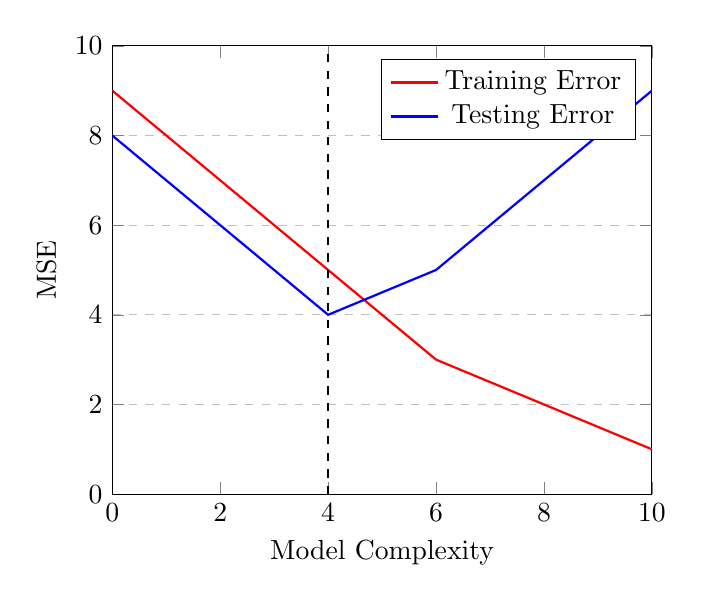
\begin{tikzpicture}
        \begin{axis}[
            xlabel={Model Complexity},
            ylabel={MSE},
            xmin=0, xmax=10,
            ymin=0, ymax=10,
            xtick={0,2,4,6,8,10},
            ytick={0,2,4,6,8,10},
            legend pos=north east,
            ymajorgrids=true,
            grid style=dashed,
        ]
        % Training error curve
        \addplot[
            color=red,
            mark=none,
            thick,
        ]
        coordinates {
            (0,9)(2,7)(4,5)(6,3)(8,2)(10,1)
        };
        \addlegendentry{Training Error}

        % Testing error curve
        \addplot[
            color=blue,
            mark=none,
            thick,
        ]
        coordinates {
            (0,8)(2,6)(4,4)(6,5)(8,7)(10,9)
        };
        \addlegendentry{Testing Error}

        % Optimal model complexity line
        \draw[dashed, thick] (axis cs:4,0) -- (axis cs:4,10);
        \node at (axis cs:4,10.5) {Optimal Model Complexity};

        \end{axis}
    \end{tikzpicture}
\end{figure}

\begin{figure}
    \centering
    \tikzsetnextfilename{cnn-pooling}
\begin{tikzpicture}

    % Draw the 5x5 image grid with a slanted effect
    \begin{scope}[canvas is xy plane at z=0]
        \node[inner sep=0, anchor=south west] (image) at (0,0) {\includegraphics[width=5cm,height=5cm]{cat.png}};
        \foreach \x in {0,1,2,3,4} {
            \foreach \y in {0,1,2,3,4} {
                \draw[fill=gray!20, opacity=0.5] (\x,\y) rectangle ++(1,1);
            }
        }
        \node at (2.5, -0.5) {5x5 Image};
    \end{scope}

    % Draw the 3x3 kernel grid
    \begin{scope}[canvas is xy plane at z=3]
        \foreach \x in {6,7,8} {
            \foreach \y in {0,1,2} {
                \draw[fill=gray!40] (\x,\y) rectangle ++(1,1);
            }
        }
        \node at (7.5, -0.5) {3x3 Kernel};
    \end{scope}

    % Draw the convolution operation arrow
    \draw[->, thick] (5, 2.5, 0) -- (6, 2.5, 3);

    % Draw the resulting 3x3 feature map grid
    \begin{scope}[canvas is xy plane at z=6]
        \foreach \x in {10,11,12} {
            \foreach \y in {0,1,2} {
                \draw[fill=gray!60] (\x,\y) rectangle ++(1,1);
            }
        }
        \node at (11.5, -0.5) {3x3 Feature Map};
    \end{scope}

    % Draw the pooling layer grid
    \begin{scope}[canvas is xy plane at z=9]
        \foreach \x in {14,15} {
            \foreach \y in {0,1} {
                \draw[fill=gray!80] (\x,\y) rectangle ++(1,1);
            }
        }
        \node at (14.5, -0.5) {2x2 Pooling};
    \end{scope}

    % Draw the pooling operation arrow
    \draw[->, thick] (13, 1.5, 6) -- (14, 1.5, 9);

    % Draw the resulting 2x2 pooled feature map grid
    \begin{scope}[canvas is xy plane at z=12]
        \foreach \x in {18,19} {
            \foreach \y in {0,1} {
                \draw[fill=gray!100] (\x,\y) rectangle ++(1,1);
            }
        }
        \node at (18.5, -0.5) {2x2 Pooled Feature Map};
    \end{scope}

    % Highlight the first convolution operation
    \begin{scope}[canvas is xy plane at z=0]
        \foreach \x in {0,1,2} {
            \foreach \y in {0,1,2} {
                \draw[fill=blue!20, opacity=0.5] (\x,\y) rectangle ++(1,1);
            }
        }
    \end{scope}

    \begin{scope}[canvas is xy plane at z=3]
        \foreach \x in {6,7,8} {
            \foreach \y in {0,1,2} {
                \draw[fill=blue!40, opacity=0.5] (\x,\y) rectangle ++(1,1);
            }
        }
    \end{scope}

    \begin{scope}[canvas is xy plane at z=6]
        \foreach \x in {10} {
            \foreach \y in {0} {
                \draw[fill=blue!60, opacity=0.5] (\x,\y) rectangle ++(1,1);
            }
        }
    \end{scope}

    % Highlight the pooling operation
    \begin{scope}[canvas is xy plane at z=6]
        \foreach \x in {10,11} {
            \foreach \y in {0,1} {
                \draw[fill=red!20, opacity=0.5] (\x,\y) rectangle ++(1,1);
            }
        }
    \end{scope}

    \begin{scope}[canvas is xy plane at z=9]
        \foreach \x in {14,15} {
            \foreach \y in {0,1} {
                \draw[fill=red!40, opacity=0.5] (\x,\y) rectangle ++(1,1);
            }
        }
    \end{scope}

    \begin{scope}[canvas is xy plane at z=12]
        \foreach \x in {18} {
            \foreach \y in {0} {
                \draw[fill=red!60, opacity=0.5] (\x,\y) rectangle ++(1,1);
            }
        }
    \end{scope}

\end{tikzpicture}
\end{figure}

\begin{figure}
    \centering
    \tikzsetnextfilename{convolution}
    \begin{tikzpicture}

        % Add background image to the 5x5 image grid
        \node[inner sep=0] (image) at (2.5, 2.5) {\includegraphics[width=5cm,height=5cm]{cat.png}};

        % Draw the 5x5 image grid
        \foreach \x in {0,1,2,3,4} {
            \foreach \y in {0,1,2,3,4} {
                \draw[fill=gray!20, opacity=0.5] (\x,\y) rectangle ++(1,1);
            }
        }

        % Label the image grid
        \node at (2.5, -0.5) {5x5 Image};

        % Draw the 3x3 kernel grid
        \foreach \x in {6,7,8} {
            \foreach \y in {0,1,2} {
                \draw[fill=gray!40] (\x,\y) rectangle ++(1,1);
            }
        }

        % Label the kernel grid
        \node at (7.5, -0.5) {3x3 Kernel};

        % Draw the convolution operation arrow
        \draw[->, thick] (4.5, 2.5) -- (5.5, 2.5);

        % Draw the resulting 3x3 feature map grid
        \foreach \x in {10,11,12} {
            \foreach \y in {0,1,2} {
                \draw[fill=gray!60] (\x,\y) rectangle ++(1,1);
            }
        }

        % Label the feature map grid
        \node at (11.5, -0.5) {3x3 Feature Map};

        % Highlight the first convolution operation
        \foreach \x in {0,1,2} {
            \foreach \y in {0,1,2} {
                \draw[fill=blue!20, opacity=0.5] (\x,\y) rectangle ++(1,1);
            }
        }

        \foreach \x in {6,7,8} {
            \foreach \y in {0,1,2} {
                \draw[fill=blue!40, opacity=0.5] (\x,\y) rectangle ++(1,1);
            }
        }

        \foreach \x in {10} {
            \foreach \y in {0} {
                \draw[fill=blue!60, opacity=0.5] (\x,\y) rectangle ++(1,1);
            }
        }

    \end{tikzpicture}
\end{figure}


\begin{figure}
    \centering
    \tikzsetnextfilename{cnn}
    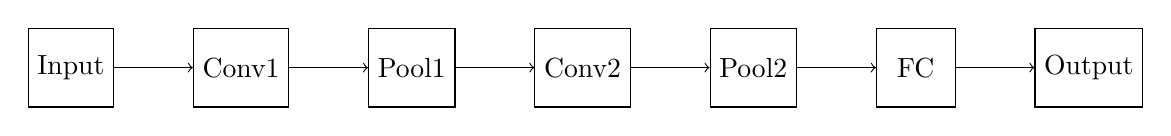
\begin{tikzpicture}

        % Input Layer
        \node[draw, minimum width=1cm, minimum height=1cm] (input) at (0,0) {Input};

        % Convolutional Layer 1
        \node[draw, minimum width=1cm, minimum height=1cm, right=of input] (conv1) {Conv1};
        \draw[->] (input) -- (conv1);

        % Pooling Layer 1
        \node[draw, minimum width=1cm, minimum height=1cm, right=of conv1] (pool1) {Pool1};
        \draw[->] (conv1) -- (pool1);

        % Convolutional Layer 2
        \node[draw, minimum width=1cm, minimum height=1cm, right=of pool1] (conv2) {Conv2};
        \draw[->] (pool1) -- (conv2);

        % Pooling Layer 2
        \node[draw, minimum width=1cm, minimum height=1cm, right=of conv2] (pool2) {Pool2};
        \draw[->] (conv2) -- (pool2);

        % Fully Connected Layer
        \node[draw, minimum width=1cm, minimum height=1cm, right=of pool2] (fc) {FC};
        \draw[->] (pool2) -- (fc);

        % Output Layer
        \node[draw, minimum width=1cm, minimum height=1cm, right=of fc] (output) {Output};
        \draw[->] (fc) -- (output);

    \end{tikzpicture}

\end{figure}




\begin{figure}
    \centering
    \tikzsetnextfilename{loss-curve}
    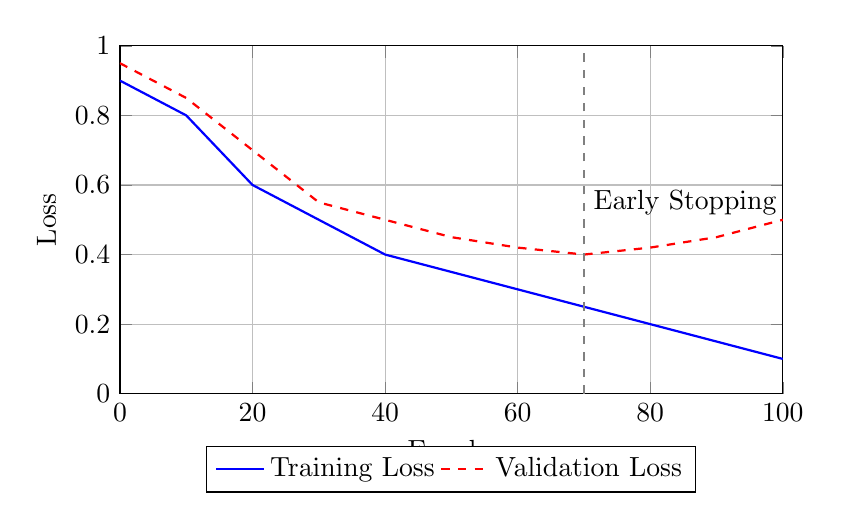
\begin{tikzpicture}
    \begin{axis}[
        xlabel={Epochs},
        ylabel={Loss},
        grid=major,
        width=10cm,
        height=6cm,
        ymin=0, ymax=1,
        xmin=0, xmax=100,
        legend style={at={(0.5,-0.15)}, anchor=north, legend columns=-1}
    ]
    \addplot[
        color=blue,
        mark=none,
        thick
    ] coordinates {
        (0, 0.9) (10, 0.8) (20, 0.6) (30, 0.5) (40, 0.4) (50, 0.35) (60, 0.3) (70, 0.25) (80, 0.2) (90, 0.15) (100, 0.1)
    };
    \addlegendentry{Training Loss}
    
    \addplot[
        color=red,
        mark=none,
        thick,
        dashed
    ] coordinates {
        (0, 0.95) (10, 0.85) (20, 0.7) (30, 0.55) (40, 0.5) (50, 0.45) (60, 0.42) (70, 0.4) (80, 0.42) (90, 0.45) (100, 0.5)
    };
    \addlegendentry{Validation Loss}
    
    \draw[dashed, gray] (axis cs:70,0) -- (axis cs:70,1);
    \node at (axis cs:70,0.55) [anchor=west] {Early Stopping};
    
    \end{axis}
    \end{tikzpicture}
\end{figure}

\begin{figure}
    \centering
    \tikzsetnextfilename{linear-regression}
    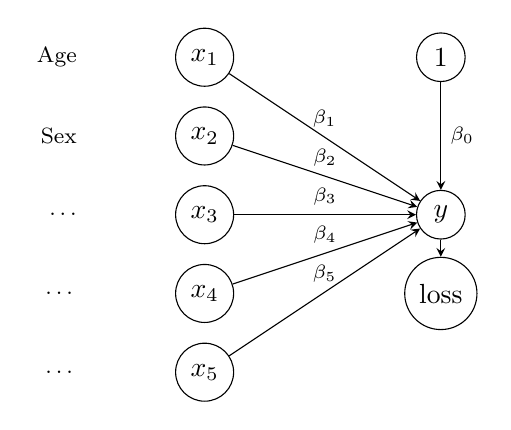
\begin{tikzpicture}[
		  % Define the style of the neural network nodes
		  neuron/.style={circle, draw, minimum size=1.5em},
		  % Define the style of the arrow between nodes
		  arrow/.style={->, >=stealth},
		  % Define the style of the weights
		  weight/.style={midway, above, font=\scriptsize},
		  % Define the style of the input labels
		  inputlabel/.style={above, font=\small},
		  % Define the style of the informative text labels
		  infolabel/.style={left, font=\footnotesize, align=center}
		  ]

		  % Input layer nodes
		  \foreach \i/\info in {1/Age, 2/Sex, 3/$\ldots$, 4/\ldots, 5/\ldots} {
		    \node[neuron] (input\i) at (0, -\i) {$x_{\i}$};
		    \node[infolabel] at (-1.5, -\i) {\info};
		  }
		  % intercept node
		  \node[neuron] (intercept) at (3, -1) {$1$};

		  % Output node
		  \node[neuron] (output) at (3, -3) {$y$};
		  \node[neuron, below of=output] (loss) {loss};

		  % Connect the nodes
		  \foreach \i in {1, ..., 5} {
		    \draw[arrow] (input\i) -- (output) node[weight] {$\beta_{\i}$};
		  }
		  \draw[arrow] (intercept) -- (output) node[weight, pos=0.5, right] {$\beta_0$};
		  \draw[arrow] (output) -- (loss) node[weight, midway, above] {};
    \end{tikzpicture}
\end{figure}

\begin{figure}
    \centering
    \tikzsetnextfilename{neural-network}
		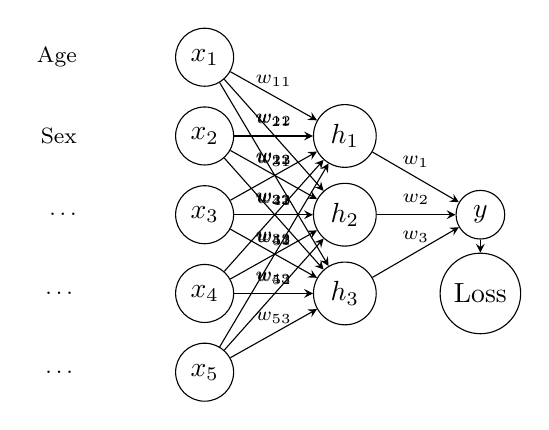
\begin{tikzpicture}[
		  % Define the style of the neural network nodes
		  neuron/.style={circle, draw, minimum size=1.5em},
		  % Define the style of the arrow between nodes
		  arrow/.style={->, >=stealth},
		  % Define the style of the weights
		  weight/.style={midway, above, font=\scriptsize},
		  % Define the style of the input labels
		  inputlabel/.style={above, font=\small},
		  % Define the style of the informative text labels
		  infolabel/.style={left, font=\footnotesize, align=center}
		  ]

		  % Input layer nodes
		  \foreach \i/\info in {1/Age, 2/Sex, 3/$\ldots$, 4/\ldots, 5/\ldots} {
		    \node[neuron] (input\i) at (0, -\i) {$x_{\i}$};
		    \node[infolabel] at (-1.5, -\i) {\info};
		  }

		  % Hidden layer nodes
		  \foreach \h [evaluate=\h as \k using {\h + 1}]in {1, 2, 3} {
		    \node[neuron, right=1cm of input\k] (hidden\h) {$h_{\h}$};
		  }

		  % Output node
		  \node[neuron, right=1cm of hidden2] (output) {$y$};
		  \node[neuron, below of=output] (loss) {Loss};

		  % Connect the nodes
		  \foreach \i in {1, ..., 5} {
		    \foreach \h in {1, 2, 3} {
		      \draw[arrow] (input\i) -- (hidden\h) node[weight] {$w_{\i\h}$};
		    }
		  }
		  \foreach \h in {1, 2, 3} {
		    \draw[arrow] (hidden\h) -- (output) node[weight] {$w_{\h}$};
		  }
		  \draw[arrow] (output) -- (loss) node[weight, midway, above] {};
		\end{tikzpicture}
\end{figure}

\end{document}
